\documentclass[12pt,a4paper]{article}
\usepackage[utf8]{vietnam}
\usepackage{amsmath,amssymb}
\usepackage{tabularx}
\usepackage{tikz}
\usetikzlibrary{calc,angles,quotes,arrows.meta,patterns}
\usepackage{xcolor}
\usepackage{enumitem}
\usepackage{fancyhdr}
\usepackage{graphicx}
\usepackage[top=1.0cm, bottom=1.0cm, left=1.2cm, right=1.2cm]{geometry}
\usepackage[dethi]{ex_test}
\SAOPTN{widthSA=3.2,heightSA=0.62}

\setlength{\headheight}{15pt}
\setlength{\parskip}{0pt}

\pagestyle{fancy}
\fancyhf{}
\rhead{\textit{Môn Toán 8 -- Đề số 09}}
\lhead{\textit{Bộ đề ôn tập Giữa học kì I}}
\cfoot{\thepage}

\begin{document}

% --- KHUNG TIÊU ĐỀ ĐỀ THI ---
\noindent
\begin{tabularx}{\linewidth}{X r}
\textbf{TRƯỜNG THCS: \dotfill} & \textbf{ĐỀ KIỂM TRA ĐỊNH KỲ GIỮA HỌC KỲ I} \\
\textbf{Họ và tên: \dotfill} & \textbf{NĂM HỌC 2026 -- 2027} \\
\textbf{Lớp: \dotfill \quad SBD: \dotfill} & \textbf{Môn: TOÁN 8} \\
\hline
\end{tabularx}
\vspace{2mm}

\begin{center}
  \textbf{\large ĐỀ ÔN TẬP GIỮA HỌC KỲ I -- ĐỀ SỐ 09}\\
  \textit{Thời gian làm bài: 90 phút (Không kể thời gian phát đề)}
\end{center}
\vspace{1mm}

% --- PHẦN I ---
\noindent\textbf{\large PHẦN I. CÂU TRẮC NGHIỆM NHIỀU PHƯƠNG ÁN LỰA CHỌN (3,0 điểm)}

\textit{Thí sinh trả lời từ câu 1 đến câu 12. Mỗi câu hỏi thí sinh chỉ chọn một phương án duy nhất.}

\vspace{1mm}
\begin{ex}
Trong các biểu thức sau, biểu thức nào là đơn thức?
\choice
{$\dfrac{1}{x} + y$}
{\True $2xy^2$}
{$(2 - x)y^2$}
{$\sqrt{x - y}$}
\end{ex}

\begin{ex}
Tích của hai đơn thức $\dfrac{1}{2}xy^3$ và $(-8x^2yz^2)$ có phần hệ số là:
\choice
{$\dfrac{1}{2}$}
{$-8$}
{\True $-4$}
{$7$}
\end{ex}

\begin{ex}
Hình thang cân là hình thang có:
\choice
{\True Hai góc kề một đáy bằng nhau}
{Hai góc đối bằng nhau}
{Hai cạnh đối bằng nhau}
{Hai đường chéo vuông góc với nhau}
\end{ex}

\begin{ex}
Kết quả khai triển biểu thức $(x - 2)(x - 2)$ là:
\choice
{$x^2 + 2x + 4$}
{$x^2 + 4x + 4$}
{$x^2 - 2x + 4$}
{\True $x^2 - 4x + 4$}
\end{ex}

\begin{ex}
Chọn câu sai trong các câu sau:
\choice
{Tứ giác có 3 góc tù, 1 góc nhọn}
{\True Tứ giác có 3 góc vuông, 1 góc nhọn}
{Tứ giác có nhiều nhất 2 góc tù, nhiều nhất 2 góc nhọn}
{Tứ giác có 3 góc nhọn, 1 góc tù}
\end{ex}

\begin{ex}
Tứ giác có hai cạnh đối song song là:
\choice
{Hình thang cân}
{\True Hình thang}
{Hình bình hành}
{Hình chữ nhật}
\end{ex}

\begin{ex}
Giá trị của biểu thức $A = x^3y + 7x^2y + 9$ tại $x = -1, y = 2$ là:
\choice
{\True $21$}
{$25$}
{$-7$}
{$-3$}
\end{ex}

\begin{ex}
Chọn đẳng thức sai trong các đẳng thức sau đây:
\choice
{$(a + b)^3 = a^3 + 3a^2b + 3ab^2 + b^3$}
{$(-a - b)^3 = -a^3 - 3a^2b - 3ab^2 - b^3$}
{\True $(-a + b)^3 = -a^3 - 3a^2b + 3ab^2 + b^3$}
{$(a - b)^3 = a^3 - 3a^2b + 3ab^2 - b^3$}
\end{ex}

\begin{ex}
Phân thức nào sau đây bằng với phân thức $\dfrac{y}{3x}$ (với giả thiết các phân thức đều có nghĩa)?
\choice
{$\dfrac{3y}{9xy^2}$}
{$\dfrac{2y^2}{9xy^2}$}
{\True $\dfrac{3y^2}{9xy}$}
{$\dfrac{3y}{9xy}$}
\end{ex}

\begin{ex}
Cho hình chóp tam giác đều có diện tích đáy bằng $6\text{ cm}^2$ và chiều cao bằng $4\text{ cm}$. Thể tích của hình chóp đó là:
\choice
{\True $8\text{ cm}^3$}
{$24\text{ cm}^3$}
{$12\text{ cm}^3$}
{$72\text{ cm}^3$}
\end{ex}

\begin{ex}
Hình thoi có chu vi bằng $20\text{ cm}$ thì độ dài cạnh của nó bằng:
\choice
{$4\text{ cm}$}
{\True $5\text{ cm}$}
{$8\text{ cm}$}
{$9\text{ cm}$}
\end{ex}

\begin{ex}
Hãy chọn câu sai:
\choice
{Tứ giác có hai cặp cạnh đối song song là hình bình hành}
{\True Hình thang có hai góc kề một đáy bằng nhau là hình bình hành}
{Tứ giác có hai cặp cạnh đối bằng nhau là hình bình hành}
{Tứ giác có hai cặp góc đối bằng nhau là hình bình hành}
\end{ex}


\vspace{1mm}
\noindent\textbf{BẢNG TRẢ LỜI TRẮC NGHIỆM PHẦN I:}
\begin{center}
\begin{tabular}{|c|c|c|c|c|c|c|c|c|c|c|c|c|}
\hline
\textbf{Câu} & \textbf{1} & \textbf{2} & \textbf{3} & \textbf{4} & \textbf{5} & \textbf{6} & \textbf{7} & \textbf{8} & \textbf{9} & \textbf{10} & \textbf{11} & \textbf{12} \\
\hline
\textbf{Chọn} & \rule{0pt}{0.65cm} & & & & & & & & & & & \\
\hline
\end{tabular}
\end{center}
\vspace{2mm}

\setcounter{ex}{0}
\noindent\textbf{\large PHẦN II. CÂU TRẮC NGHIỆM ĐÚNG SAI (2,0 điểm)}

\textit{Thí sinh trả lời câu 1 và câu 2. Trong mỗi ý a), b), c), d) ở mỗi câu, thí sinh chọn đúng hoặc sai.}

\vspace{1mm}
\begin{ex}
Cho hai đa thức $P = x(x - 2y) + y(y + 2x)$ và $Q = x^2 - 4y^2$. Xét tính đúng sai của các mệnh đề sau:
\choiceTF
{\True Rút gọn đa thức $P$ ta được $x^2 + y^2$}
{Tại $x = 3$ và $y = 4$, giá trị của đa thức $P$ bằng $49$}
{\True Phân tích đa thức $Q$ thành nhân tử ta được $(x - 2y)(x + 2y)$}
{\True Với $x = 2y$ và $y \neq 0$, phân thức $\dfrac{P}{Q}$ không xác định}
\end{ex}

\begin{ex}
Cho biểu thức $A = \dfrac{x^2 - 6x + 9}{x^2 - 9}$ với $x \neq \pm 3$. Xét tính đúng sai của các mệnh đề sau:
\choiceTF
{\True Biến đổi tử thức $x^2 - 6x + 9$ thành bình phương của một hiệu ta được $(x - 3)^2$}
{\True Phân tích mẫu thức $x^2 - 9$ thành nhân tử ta được $(x - 3)(x + 3)$}
{Kết quả rút gọn của biểu thức $A$ là $\dfrac{x + 3}{x - 3}$}
{\True Tại $x = 5$, giá trị của biểu thức bằng $\dfrac{1}{4}$}
\end{ex}


\noindent\textbf{BẢNG TRẢ LỜI PHẦN II:}
\begin{center}
\begin{tabular}{|c|c|c|c|c||c|c|c|c|c|}
\hline
\textbf{Câu 1} & \textbf{a)} & \textbf{b)} & \textbf{c)} & \textbf{d)} & \textbf{Câu 2} & \textbf{a)} & \textbf{b)} & \textbf{c)} & \textbf{d)} \\
\hline
\textbf{Đ/S} & \rule{0pt}{0.6cm} & & & & \textbf{Đ/S} & & & & \\
\hline
\end{tabular}
\end{center}
\vspace{2mm}

\setcounter{ex}{0}
\noindent\textbf{\large PHẦN III. CÂU HỎI TRẢ LỜI NGẮN (2,0 điểm)}

\textit{Thí sinh trả lời câu 1 và câu 2. Điền kết quả vào ô trống tương ứng.}

\vspace{1mm}
\begin{ex}
Tìm $x$, biết: $x^2 - 16 - 2(x + 4) = 0$. \shortans{$x = -4$ hoặc $x = 6$}
\end{ex}

\begin{ex}
Cho hình thoi $ABCD$ có $\widehat{A} = 60^\circ$ và độ dài cạnh $AB = 5\text{ cm}$. Tính độ dài đường chéo $BD$. \shortans{$5\text{ cm}$}
\end{ex}


\setcounter{ex}{0}
\noindent\textbf{\large PHẦN IV. TỰ LUẬN (3,0 điểm)}

\textit{Thí sinh trình bày chi tiết lời giải vào giấy làm bài.}

\vspace{1mm}
\begin{ex} (1,0 điểm)
Thực hiện phép tính:
\begin{enumerate}[label=\textbf{\alph*)}, leftmargin=0.8cm, itemsep=2pt]
\item (0,35 điểm) $2x(3x - y) - (6x^2 - 2xy + 3)$
\item (0,35 điểm) $(12x^3y^2 - 9x^2y^3 + 3x^2y^2) : (3x^2y)$
\item (0,3 điểm) $(x + 2)^2 - (x - 2)^2$
\end{enumerate}
\end{ex}
\vspace{0.5mm}

\begin{ex} (0,75 điểm)
Tìm $x$, biết:
\begin{enumerate}[label=\textbf{\alph*)}, leftmargin=0.8cm, itemsep=2pt]
\item (0,35 điểm) $2x(x - 3) - 2x^2 = 10$
\item (0,4 điểm) $(x + 1)^2 - (x - 2)(x + 2) = 9$
\end{enumerate}
\end{ex}
\vspace{0.5mm}

\begin{ex} (0,75 điểm)
Một khối bê tông có dạng hình chóp tứ giác đều (đáy là hình vuông) có cạnh đáy $a = 0{,}5\text{ m}$ và chiều cao $h = 0{,}6\text{ m}$.
\begin{center}
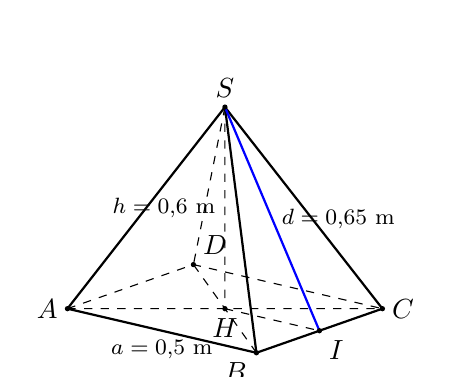
\begin{tikzpicture}[scale=0.8, >=stealth]
  \coordinate (A) at (0,0);
  \coordinate (B) at (3,-0.7);
  \coordinate (C) at (5,0);
  \coordinate (D) at (2,0.7);
  \coordinate (H) at ($(A)!0.5!(C)$);
  \coordinate (S) at ($(H)+(0,3.2)$);
  \coordinate (I) at ($(B)!0.5!(C)$);
  \draw[dashed] (A)--(D)--(C);
  \draw[dashed] (S)--(D);
  \draw[dashed] (A)--(C) (B)--(D);
  \draw[dashed] (S)--(H);
  \draw[dashed] (H)--(I);
  \draw[thick] (S)--(A)--(B)--(C)--(S);
  \draw[thick] (S)--(B);
  \draw[thick, blue] (S)--(I);
  \fill (A) circle (1.2pt) node[left] {$A$};
  \fill (B) circle (1.2pt) node[below left] {$B$};
  \fill (C) circle (1.2pt) node[right] {$C$};
  \fill (D) circle (1.2pt) node[above right] {$D$};
  \fill (S) circle (1.2pt) node[above] {$S$};
  \fill (H) circle (1.2pt) node[below] {$H$};
  \fill (I) circle (1.2pt) node[below right] {$I$};
  \node[left] at ($(S)!0.5!(H)$) {\footnotesize $h = 0{,}6\text{ m}$};
  \node[below] at ($(A)!0.5!(B)$) {\footnotesize $a = 0{,}5\text{ m}$};
  \node[right] at ($(S)!0.5!(I)$) {\footnotesize $d = 0{,}65\text{ m}$};
\end{tikzpicture}
\end{center}
\begin{enumerate}[label=\textbf{\alph*)}, leftmargin=0.8cm, itemsep=2pt]
\item (0,4 điểm) Tính thể tích khối bê tông.
\item (0,35 điểm) Người ta muốn sơn bốn mặt xung quanh của khối bê tông này. Biết chiều cao trung đoạn của hình chóp là $d = 0{,}65\text{ m}$. Tính diện tích bề mặt cần sơn.
\end{enumerate}
\end{ex}
\vspace{0.5mm}

\begin{ex} (0,5 điểm)
Tìm giá trị nhỏ nhất của biểu thức: $A = x^2 - 4x + y^2 + 6y + 15$.
\begin{enumerate}[label=\textbf{\alph*)}, leftmargin=0.8cm, itemsep=2pt]
\item (0,5 điểm) Tìm giá trị nhỏ nhất của $A$.
\end{enumerate}
\end{ex}
\vspace{0.5mm}


\begin{center}
\rule{4cm}{0.4pt}\\
\textit{--- HẾT ---}
\end{center}
\end{document}
